
\(f(x) = x^3 - 6x^2 + 9x + 1\).

\subsection*{1.}

La fonction polynôme \(f\) est dérivable sur \(\mathbb{R}\) et sur \([-1\,;\,5]\), et sa dérivée est :
\[
f'(x) = 3x^2 - 12x + 9 = 3(x^2 - 4x + 3).
\]

\subsection*{2.}

Le nombre 1 est une racine évidente du trinôme \(x^2 - 4x + 3\), et comme le produit des racines est \(\dfrac{c}{a} = \dfrac{3}{1} = 3\), l'autre racine est 3.

On sait que \(x^2 - 4x + 3 = (x - 1)(x - 3)\), donc \(f'(x) = 3(x - 1)(x - 3)\).

\subsection*{3.}

Le trinôme est du signe de \(a = 1 > 0\), donc positif sauf sur l'intervalle \(\left]1\,;\,3\right[\).  

Il en résulte que sur l'intervalle \([-1\,;\,5]\) :
\[f(-1) = -1 - 6 - 9 + 1 = -15 \quad ; \quad f(1) = 1 - 6 + 9 + 1 = 5\]
\[f(3) = 27 - 54 + 27 + 1 = 1 \quad ; \quad f(5) = 125 - 150 + 45 + 1 = 21\]
\begin{center}
\begin{tikzpicture}
\tkzTabInit[lgt=2.5, espcl=2]{$x$ / 1, {Signe de $f'(x)$} / 1, {$f$} / 2}{${-1}$, ${1}$, ${3}$, ${5}$}
\tkzTabLine{,+,0,-,0,+,}
\tkzTabVar{-/{$-15$},+/{$5$},-/{$1$},+/{$21$}}{/}
\end{tikzpicture}
\end{center}

\subsection*{4.}

On sait qu'une équation de la tangente \(\mathcal{T}\) à la courbe représentative de la fonction \(f\) au point d'abscisse \(0\) est :
\[
M(x\,;\,y) \in \mathcal{T} \iff y - f(0) = f'(0)(x - 0).
\]
Avec \(f(0) = 1\) et \(f'(0) = 9\), on obtient :
\[
M(x\,;\,y) \in \mathcal{T} \iff y = 9x + 1.
\]

\subsection*{5.}

Si une autre tangente est parallèle à \(\mathcal{T}\), son coefficient directeur est égal à 9.

Or,
\begin{align*}
f'(x) &= 9 \\
3(x^2 - 4x + 3) &= 9 \\
x^2 - 4x + 3 &= 3 \\
x^2 - 4x &= 0 \\
x(x - 4) &= 0.
\end{align*}

On retrouve \(x = 0\) pour la tangente \(\mathcal{T}\), et \(x = 4\), pour lequel :
\[
f(4) = 64 - 96 + 36 + 1 = 5.
\]  
La tangente à la courbe représentative de la fonction \(f\) au point \(B(4\,;\,5)\) est parallèle à \(\mathcal{T}\).

